\chapter{The problem}
\label{chp:problem}
Following~\cite{mariotto2022}, the HO corrector magnets have been designed to produce five different multipolar field orders (quadrupole, sextupole, octapole, decapole, and dodecapole). Tested at cryogenic temperature, the magnets are powered to evaluate their performances and thermal stability up to the nominal operating condition. During magnet powering, spontaneous quench transitions in the superconducting coil volume can occur due to mechanical instability of the winding or stress induced by the electromagnetic Lorentz forces acting on the conductors. Each magnet is protected using a classical resistive voltage detection system and discharged on an external dumping resistance to extract most of the stored magnetic energy from the magnet to prevent any material damage. Limited to analyzing only two separate voltage signals connected in parallel to the coils, the quench detection system can only evaluate if a quench development occurred in half of the magnet coils without the possibility to localize precisely which superconducting winding started the transition to the normal conducting state. To retrieve this information and evaluate if a possible degradation of the coil has occurred, a magnetic field measurement-based model has been proposed analyzing the residual magnetic field quality produced by the non-quenched superconducting coils in the magnet after the quench event. The original work proposed a study specific to quadrupoles, since they gave the majority of the positives (quench events), which have been used as the subject of this analysis, therefore ignoring all other configurations focusing only on the five quadrupoles of the series production from MQSXF1 to MQSXF6.
\begin{figure}[h!]
	\centering
	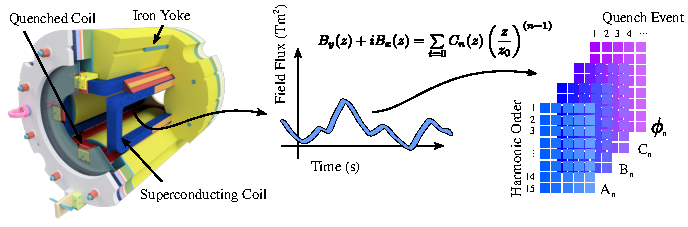
\includegraphics[width=\linewidth]{img/FieldProcedure.pdf}
	\caption{Sketch of the magnetic field measurements after a quench event for the quadrupole magnet and dataset obtained for each quench event measurement.}
	\label{fig:FieldMeasurement}
\end{figure}
As a result of the magnets test campaign, $279$ events, after the magnet discharge (quench event) or equivalent at zero operating current (non-quench event), were analyzed sampling the magnetic field in the magnet bore volume using a magnetic field rotating shaft.

For each event, 60 samples of measured harmonic coefficients have been measured and averaged to obtain a single set of $15$ different magnetic field harmonics coefficients which contain all the information of the produced magnetic field quality (see Fig.~\ref{fig:FieldMeasurement}). Recalling that these coefficients are expressed as complex numbers, the information have been organized in terms of the following four attributes, in which the suffix $n \in \{1, \dots,  15\}$ is related to a specific harmonic:
\begin{itemize}
	\item the imaginary part \an, of the $n^\text{th}$ field harmonic coefficient;
	\item the real part \bn, of the $n^\text{th}$ field harmonic coefficient;
	\item the absolute value \cnmod, of the $n^\text{th}$ field harmonic coefficient;
	\item the phase \phin, of the $n^\text{th}$ field harmonic coefficient.
\end{itemize}
In the experiment generating data, the magnets were mounted skewed: as a consequence, the $A_n$ feature was supposed to be highly informative since they are directly correlated with the rotational position of the quenched coil in the magnet assembly. The absolute values $|C_n|$ would be a valuable feature for \qrp{} and not for \qlp{} since two different configurations with the same number of quenched coils but different angular positions would give the same harmonic content and different phases. Each measurement was coupled with a \emph{label} encoded as follows:
\begin{itemize}
	\item a simple binary flag for \qrp, where $1$ means that a quench has happened, while $0$ characterizes the normal working conditions of the superconductor;
	\item four binary flags for \qlp, each describing a  coil and stating whether or not a quench happened within it, using the same encoding as in previous point.
\end{itemize}
We remark here that the labels for \qrp\ were reasonably balanced: namely, the number of non-quench events was of $87$ while the number of quench events was of $192$; concerning \qlp, on the other hand, every coil has a different distribution: as detailed in Table~\ref{tab:balance}, the proportion of quench over non-quench events roughly ranges from $30\%$ to $50\%$. It is important to notice that the sum of all quench events for \qlp\ is not $192$, since one quench event for \qrp\ could have been caused by up to three different coils (e.g., coils 0, 1 and 3) quenching at the same time.

\begin{table}[h]
	\caption{Label distribution for the various coils in \qlp.}\label{tab:balance}

	\bigskip
	\setlength{\tabcolsep}{6pt}
	\centering
	\begin{tabular}{ccc}
		\toprule
		\textbf{Coil} & \textbf{Quench} & \textbf{Non-quench} \\
		\midrule
		0             & 68              & 211                 \\
		1             & 96              & 183                 \\
		2             & 79              & 200                 \\
		3             & 73              & 206                 \\
		\bottomrule
	\end{tabular}
\end{table}

In the following chapters we will not be using attributes in their entirety, in most cases the
datasets will be aggregating the best harmonics for a certain attribute (e.g., harmonics $2$ and
$12$ for attribute \an). We will be referring to these as sub-views of an attribute.

The objective of the thesis was to find machine learning models capable of:
\begin{enumerate}
	\item Recognizing whether the magnet underwent a quench event during operation, we will refer
	      to it as Quench Recognition Problem (\qrp) from now on, and will be treated in
	      \Cref{chp:qrp},
	\item Recognize, if the superconductor quenched, which coil(s) transitioned; we will refer to
	      it as Quench Localization Problem (\qlp) from now on, and it will be treated in
	      \Cref{chp:qlp}.
\end{enumerate}
The models chosen to solve \qrp\ and \qlp\ had to be both reliable and highly explainable to favour
further study of quench phenomenon on High-Order corrector magnets.

\section{Model selection and model testing procedures}
Reproducibility is a key property of any experiment, to cover the basics, we set the seed for all
random number generators to the same value, and we used shared pipelines for all our experiments.

Sub-views are built using a common pipeline that generates three different datasets, serialized
for later reuse:
\begin{itemize}
	\item The \emph{merged} dataset, \dm, which constructs a single table out of all the
	      measurements done on the attribute(s) for the different magnets. Before serialization, the
	      data is standardized using an instance of the StandardScaler class, contained in
	      scikit-learn, trained on the dataset just created (minus the label column(s)).
	\item The \emph{blind-test} dataset, \db, contains a small part of the overall data available to us
	      ($29$ samples), these samples were kept locked until the experiments were considered
	      complete. Using the blind-test set we performed a final test on the models to see
	      how well the performance generalize on unseen data.
	\item The \emph{reduced} dataset, \dr, contains the rest of the samples, $250$ in total,
	      and is the main set used to perform experiments.
\end{itemize}

Model selection and testing were carried out using Nested Cross Validation (\ncv). \ncv\ is suitable
for situations in which the data is not abundant~\cite{Larracy2021} due to its heavy reuse, enabling
model selection and testing, while also giving less biased performance estimates by averaging the
results on $k$ different folds, in the following section we will do a rapid excursus on how the
cross-validation procedure works.

\subsubsection{Cross Validation}
In \Cref{chp:ml} we talked about the simple train-test splitting procedure, now we will introduce an
alternative technique for splitting that gives us a powerful tool to prevent overfitting and get
less biased performance measures while also doing hyperparameter selection.

In general, given a dataset $D$, $k$-fold \cv~\cite{ZhouZhi-Hua2021ML} is a technique for splitting
a dataset in $k$ different folds $\fold{i}, i \in \{1, \ldots, k\}$, the folds are non-overlapping
and about the same size, therefore $\fold{i} \cap \fold{j} = \emptyset \hspace{5pt} \forall i, j \in
	\{1, \ldots, k\}, i \neq j$, and the union of all the folds is the original dataset ($\bigcup_{i \in \{1, \ldots, k\}} \fold{i} = D$).

\medskip

In the framework of train-test splitting, if we used the procedure outlined in \Cref{chp:ml}, we
would split the original dataset into the training set $T$ and the generalization set $G$, train
$\model$ on $T$ and then test the performance on $G$. While this is a perfectly acceptable procedure
to gather performance metrics for a model it doesn't give us any certainty on how reliable the
obtained metrics actually are.


By measuring performance on different folds (each one is a training and testing procedure separate
from others), we get a more complete vision of the model performance, allowing us to recognize pathological
situations, like cases in which the standard deviation of the fold performance is very wide. To
understand how the folds are structured, let's consider an example in which $5$-fold \cv\ is
computed on a dataset containing $250$ samples: $5$ different models are generated, each time it
trained on $200$ samples and then tested on the remaining $50$ samples (the testing fold changes
with every iteration).

The number of folds to be used for \cv\ becomes another hyperparameter of the problem, since it
depends on many factors like the amount of available data or the required reliability of performance
reads. A large value of $k$ will increase the number of folds the model is trained and tested on,
increasing the robustness of the performance estimation at the expense of computational complexity
(e.g., Leave One Out \cv\ is an example of such approaches, in~\cite{shao2016} a more efficient
approach to the technique is discussed); too small a value of $k$ makes the \cv\ less robust but more efficient (classic values of $k$ for most practical uses are $5, 10, 20$).

\medskip

Let us now move to a more complicated environment in which we need, given a base model, to do model
selection, do model training and finally do model testing. We can na\"ively tripartition dataset $D$:
\begin{itemize}
	\item \emph{Training set} $T$,
	\item \emph{Validation set} $V$, this set of samples will be used to test the performance of the
	      model found after the training step,
	\item \emph{Generalization set} $G$, after the model is retrained on $T + V$ the performance are
	      tested on $G$ to see if the model is capable of generalizing effectively.
\end{itemize}

Once again we cannot guarantee that:
\begin{inparaenum}[(i)]
	\item the chosen model is the best one,
	\item the performance metrics obtained from the single generalization fold are actually reliable.
\end{inparaenum}
To address the issue we can substitute each procedure with $k$-fold \cv, one nested inside of each
other, the \emph{inner} is used to do model selection, the \emph{outer} is used to test performance
for the model just generated. To get a better understanding of the Nested cross-validation procedure
(\ncv) just introduced let us consider a $5 \times 5$ \ncv\ procedure applied to a dataset of $250$
samples(an outline of the \ncv\ procedure is shown in \Cref{fig:nested-cv}).
\begin{itemize}
	\item The data is first split into $5$ folds of $50$ samples. One fold of $50$ samples will
	      be kept on the side for the generalization test, the remaining $200$ samples will be used to do both training and model selection;
	\item The training set is now split again in $5$ folds, $160$ samples will be used to do
	      model selection (therefore hyperparameter space search), $40$ samples will be used
	      to validate the performance that has been found;
	\item The model found at the previous step is retrained on the whole $200$ training samples and then
	      the performance are tested on the fold that was kept aside in the first step.
\end{itemize}
\begin{figure}[!t]
	\centering
	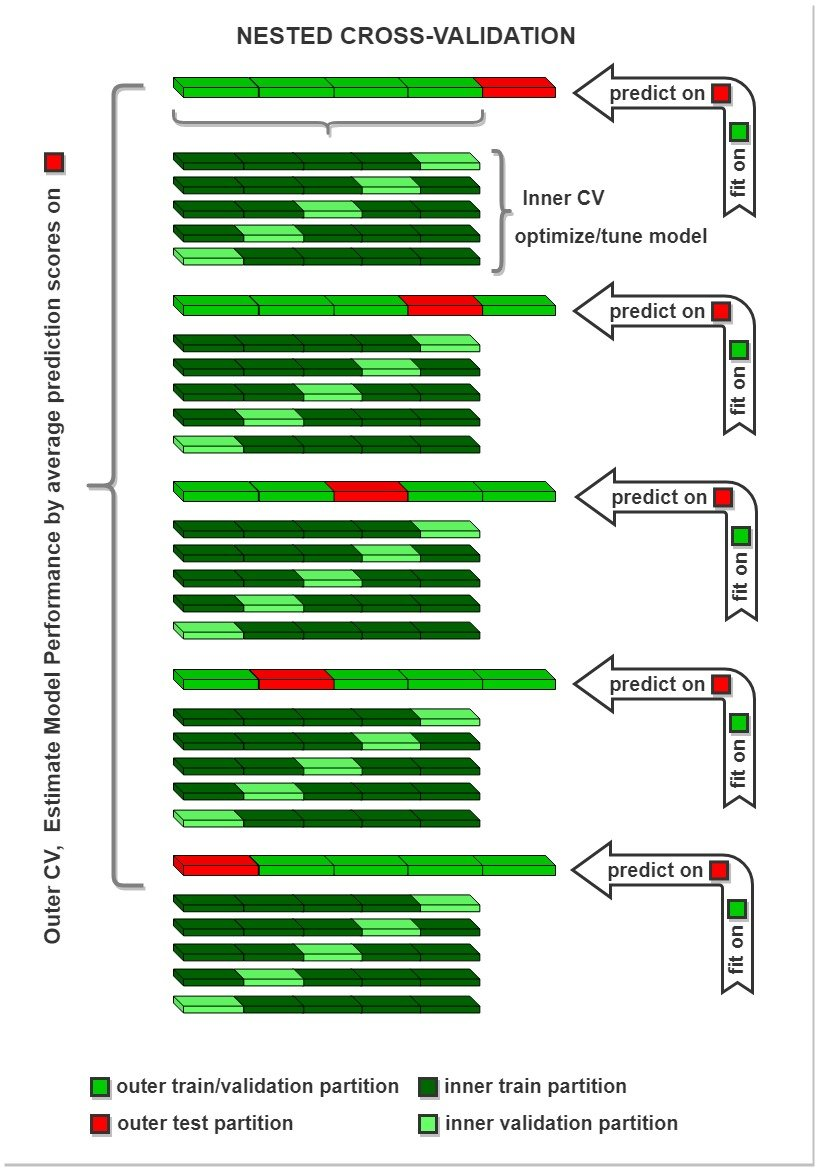
\includegraphics[scale=.3]{./img/nested-cv.png}
	\caption{Visualization of the nested cross validation procedure taken from~\cite{lavasa2021}}
	\label{fig:nested-cv}
\end{figure}

Once the \ncv\ procedure terminates we will get $k$ different models, since the fine-tuned models
are statistically equivalent, we can choose which one to keep using the heuristic that fits our
objectives the best.

The closing section for this chapter will contain a summarization of the experimental setup.

\section{Experimental setup}
The project was developed using the latest version of the Python programming language (3.10.12 at the moment of writing), All experiments have been executed using Python 3.10.12 (the latest version at the time of writing), using the following libraries: scikit-learn (release 1.5.2) for data preprocessing and model training and evaluation, numpy (release 2.2.3) for efficient data storage, and Pandas (release 2.2.3) for data management. These libraries have been handled through the pip package manager (release 25.0.1) and used within a virtual environment.

\medskip

The seeds from the various random number generators have been set to the common value of
\href{https://www.google.com/search?q=the+answer+to+life+the+universe+and+everything&num=10&client=firefox-b-d&sca_esv=a81abf9bb67ffd9b&sxsrf=AHTn8zo6RKep_zuEvIhJb5nuAGh5xAERLg\%3A1739739141586&ei=BVCyZ_C9I9mLi-gP7e-B8Ac&oq=the+answer+to+&gs_lp=Egxnd3Mtd2l6LXNlcnAiDnRoZSBhbnN3ZXIgdG8gKgIIADIIEAAYgAQYywEyCBAAGIAEGMsBMgUQABiABDIIEAAYgAQYywEyCBAAGIAEGMsBMggQABiABBjLATIIEAAYgAQYywEyCBAAGIAEGMsBMggQABiABBjLATIIEAAYgAQYywFIjCJQqQlYiRlwA3gBkAEAmAFuoAHICaoBBDExLjO4AQPIAQD4AQGYAhGgAv0JwgIKEAAYsAMY1gQYR8ICChAjGIAEGCcYigXCAgsQABiABBixAxiDAcICCxAuGIAEGLEDGIMBwgIOEC4YgAQYsQMY0QMYxwHCAg4QLhiABBixAxiDARiKBcICERAuGIAEGLEDGNEDGIMBGMcBwgIMECMYgAQYExgnGIoFwgIEECMYJ8ICDRAuGIAEGEMY1AIYigXCAgoQABiABBhDGIoFwgIOEC4YgAQYxwEYjgUYrwHCAgoQLhiABBhDGIoFwgIIEC4YgAQYsQPCAggQABiABBixA8ICCxAuGIAEGLEDGNQCwgIFEC4YgATCAggQLhiABBjLAcICCxAuGIAEGNEDGMcBmAMAiAYBkAYIkgcEMTIuNaAHrboC&sclient=gws-wiz-serp}{42} to prevent too much deviation in the experiments.

\medskip

The original contained $279$ samples, for \qrp, each sample consisted of $15$ harmonics and a Label
stating whether the sample represents a quench event ($1$) or not ($0$), for \qlp, each sample had $4$ different
labels associated to it representing whether one of the coils ($0$ for East, then: North, West and
South) quenched ($1$) or not ($0$).

Every splitting operation was performed by stratifying on the labels, in the case of \qlp, if the
labels were more than one, we used a multi-class stratification technique, detailed in (\cite{skmlearn}).

\medskip

Experiments were conducted on three different computers running different architectures and
different operating systems, but the results did not change due to the standard-oriented approach,
\Cref{tbl:computers} for a summary of the computers we used.
\begin{table}[t]
	\caption{System configuration used for our experiments. Core count values are detailed as number
		of CPU cores and threads, while frequency is expressed in the base and boost specifications.
		Finally, the CPU cache size is shown for the L1, L2 and L3 levels, where
		available.}\label{tbl:computers}

	\bigskip

	\centering
	\setlength{\tabcolsep}{4pt}
	\begin{tabular}{lccc}
		\toprule
		                     & \textbf{Pigna}        & \textbf{Mattone}         & \textbf{Topone}    \\
		\midrule
		\textbf{Model}       & Macbook Pro           & Custom build             & Dell XPS 8700      \\
		\textbf{CPU}         & i$5$ $5287\textsc{u}$ & Ryzen 7 $3700\textsc{x}$ & i$7$ $4770$        \\
		\textbf{Core count}  & $2\cc / 2\tds$        & $8\cc / 16\tds$          & $4\cc /
		8\tds$                                                                                       \\
		\textbf{Launch Date} & Q$1$ 2015             & Q$2$ 2019                & Q$2$ 2013          \\
		\textbf{Frequency}   & $2.90 / 3.30$ \ghz    & $4.125 / 4.40$ \ghz      & $3.40 / 3.90$ \ghz \\
		\textbf{Cache}       & $3$ \mb               & $0.512 / 4 / 32$ \mb     & $8$ \mb            \\
		\textbf{TDP}         & $28$ \w               & $84$ \w                  & $65$ \w            \\
		\textbf{RAM}         & $8$ \gb               & $16$ \gb                 & $16$ \gb           \\
		\textbf{OS}          & Pop!\_OS $22.04$ LTS  & Pop!\_OS $22.04$ LTS     & Fedora $39$        \\
		\bottomrule
	\end{tabular}
\end{table}
Experiments were dispatched on different systems based on the expected computational load.

Model selection was handled by doing a partial exploration of the parameter space via a grid search algorithm (GridSearchCV in scikit-learn), for each model we
defined a custom parameter grid (shown in \Cref{tbl:params}).

\begin{table}[t]
	\caption{Hyperparameters which we have tuned during the model training phase.} \label{tbl:params}

	\bigskip

	\centering
	\setlength{\tabcolsep}{6pt}
	\begin{tabular}{llc}
		\toprule
		\textbf{Model}       & \textbf{Hyperparameter}                                           & \textbf{Values}                        \\
		\midrule
		\multirow{5}{*}{DT}  & impurity criterion                                                & gini, entropy, log loss                \\
		                     & max depth                                                         & $2, 3, 4, 5$                           \\
		                     & min impurity decrease                                             & $0.001, 0.01, 0.05$                    \\
		                     & max features                                                      & None, $0.5, 0.75$                      \\
		                     & min samples leaf                                                  & $5, 10, 20$                            \\
		\midrule
		\multirow{2}{*}{RF}  & n. of trees                                                       & $2, 3, 5, 10$                          \\
		                     & \multicolumn{2}{l}{$+$ the same hyperparameters and values of DT}                                          \\
		\midrule
		\multirow{5}{*}{SVC} & $C$                                                               & $0.1, 1, 10, 100, 1000$                \\
		                     & $\gamma$                                                          & scale, auto, $0.001, 0.01, 0.1, 1, 10$ \\
		                     & degree                                                            & $2, 3, 4, 5$                           \\
		                     & $c_0$                                                             & $0, 0.1, 0.5, 1$                       \\
		                     & kernel                                                            & linear, poly sigmoid, rbf              \\
		\bottomrule
	\end{tabular}
\end{table}

All of the models have been tested on a suite of scorers meant to give us a more complete
understanding of how well the model is performing, the metrics are explained here below and, as
usual, by positive (negative) sample we mean a sample having label $1$ ($0$), and by true (false)
positive we mean a correctly classified positive (negative) sample:
\begin{itemize}
	\item \emph{Accuracy} (Acc): fraction of correct predictions,
	\item \emph{Precision} (Prc): number of true positives over number of positive predictions,
	\item \emph{Recall} (Rec): number of true positives over number of positive items,
	\item \emph{F1 score} (F1): harmonic mean between Precision and Recall,
	\item \emph{Inverse recall} (Irec): number of true negatives over number of negative items,
	\item \emph{ROC AUC} (RAUC): area under the receiver operating characteristic curve.
\end{itemize}
The main metric of our suite is going to be accuracy.





